%! TEX root = ../main.tex
% ==============================================================
% IMMUTABLE — generated automatically, do not edit this block
%
% — Provenance ───────────────────────────────────────────────────
%   script            : plotter.py::plot_frequency_spectrum
%   computed_in       : 
%   plot_type         : spectrum_psd
%   data_class        : 
%   generated_at      : 2026-04-29T09:47:57
%   findings_doc      : 
%
% — Thesis context ──────────────────────────────────────────────
%   chapter           : 04
%   caption_label     : fig:ch04_wind_psd
%   caption_short     : 
%
% — Filters ────────────────────────────────────────────────────
%   panel             : 
%   wind              : 
%   amplitude [V]     : 
%   frequency [Hz]    : 
%   probes            : 9373/170, 12400/250, 9373/340, 8804/250
%   run_category      : 
%   quality_flag      : 
%   mooring           : 
%
% — Data provenance ────────────────────────────────────────────
%   n_runs            : 37
%   in_probes_used    : 9373/170+9373/340
%   out_probes_used   : 11800/250, 12400/250
%   probe_configs     : march2026_better_rearranging, march2026_rearranging
%   non_final_config_n: 5
%   datasets        :
%     PROCESSED-20260326-ProbePos4_31_FPV_2-tett6roof-under9Mooring-height100-lowrange
%     PROCESSED-20260327-ProbePos4_31_FPV_2-tett6roof-under9Mooring30-height100-lowrange
%   run_paths       :
%     (omitted — aggregate over > threshold runs, see datasets)
%
% — Method / numerical parameters ─────────────────────────────
%   grouper           : 
%   collapse_panels   : 
%   fft_window_hz     : 
%   extra_params      : 
%
% — Summary stats cited in caption ────────────────────────────
%   (none registered — pass extra_stats=... to build_fig_meta)
%
% — Subfigures available ───────────────────────────────────────
%     FIGURES/ch04_wind_psd.pdf
%     FIGURES/ch04_wind_psd.pdf
%     FIGURES/ch04_wind_psd.pdf
%     FIGURES/ch04_wind_psd.pdf
% ── end immutable block ─────────────────────────────────────────
\begin{figure}[htbp]
  \centering
  \begin{subfigure}[b]{0.48\linewidth}
    \centering
    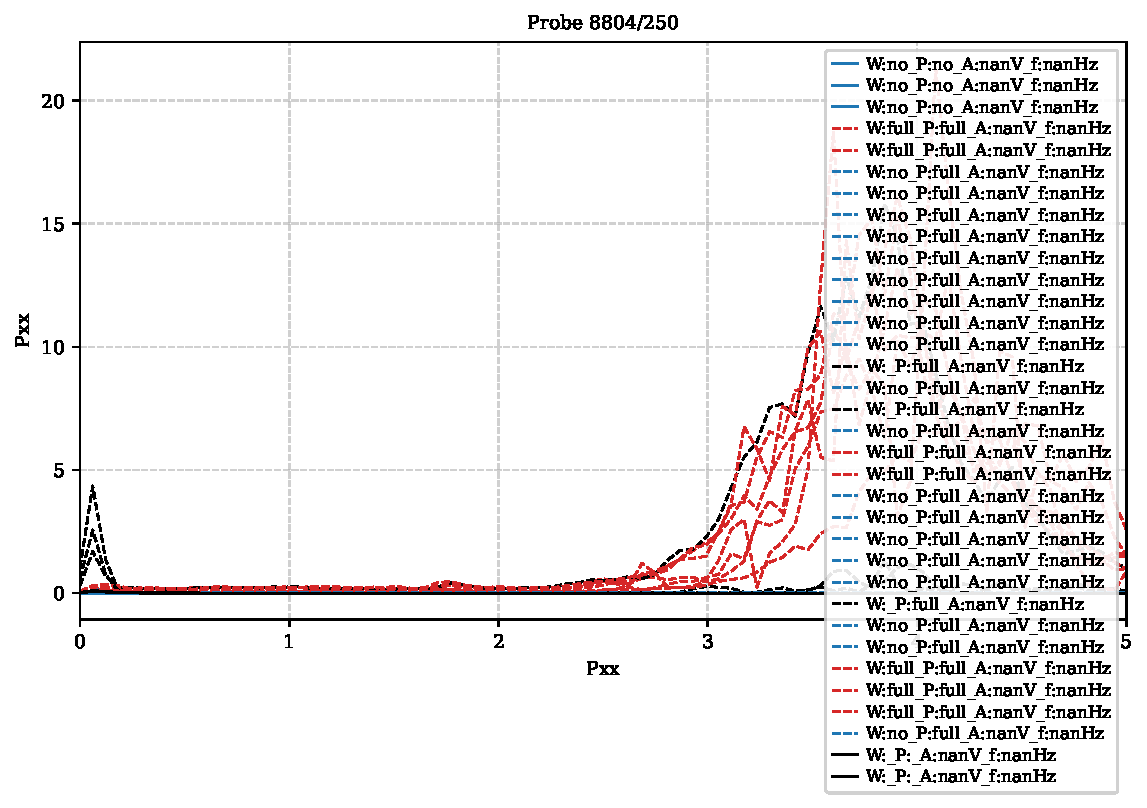
\includegraphics[width=\linewidth]{FIGURES/ch04_wind_psd.pdf}
    \caption{TODO}
    \label{fig:ch04_wind_psd}
  \end{subfigure}
  \hfill
  \begin{subfigure}[b]{0.48\linewidth}
    \centering
    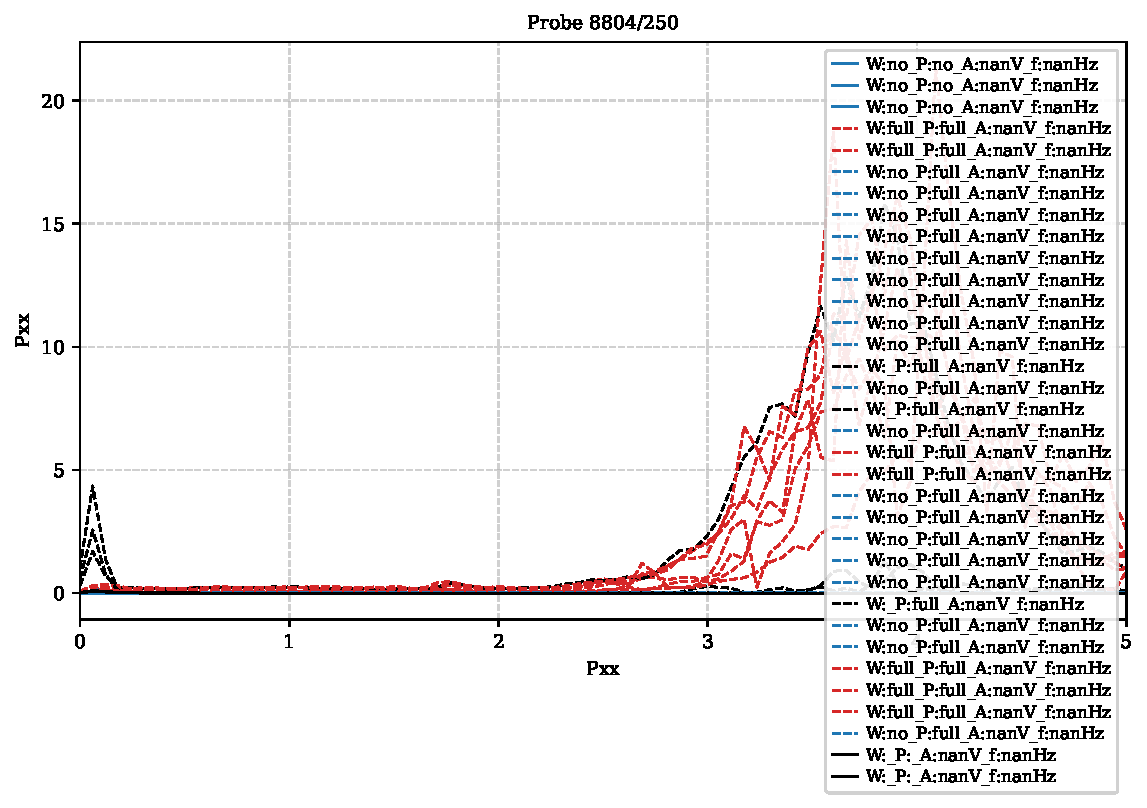
\includegraphics[width=\linewidth]{FIGURES/ch04_wind_psd.pdf}
    \caption{TODO}
    \label{fig:ch04_wind_psd}
  \end{subfigure}
  \hfill
  \begin{subfigure}[b]{0.48\linewidth}
    \centering
    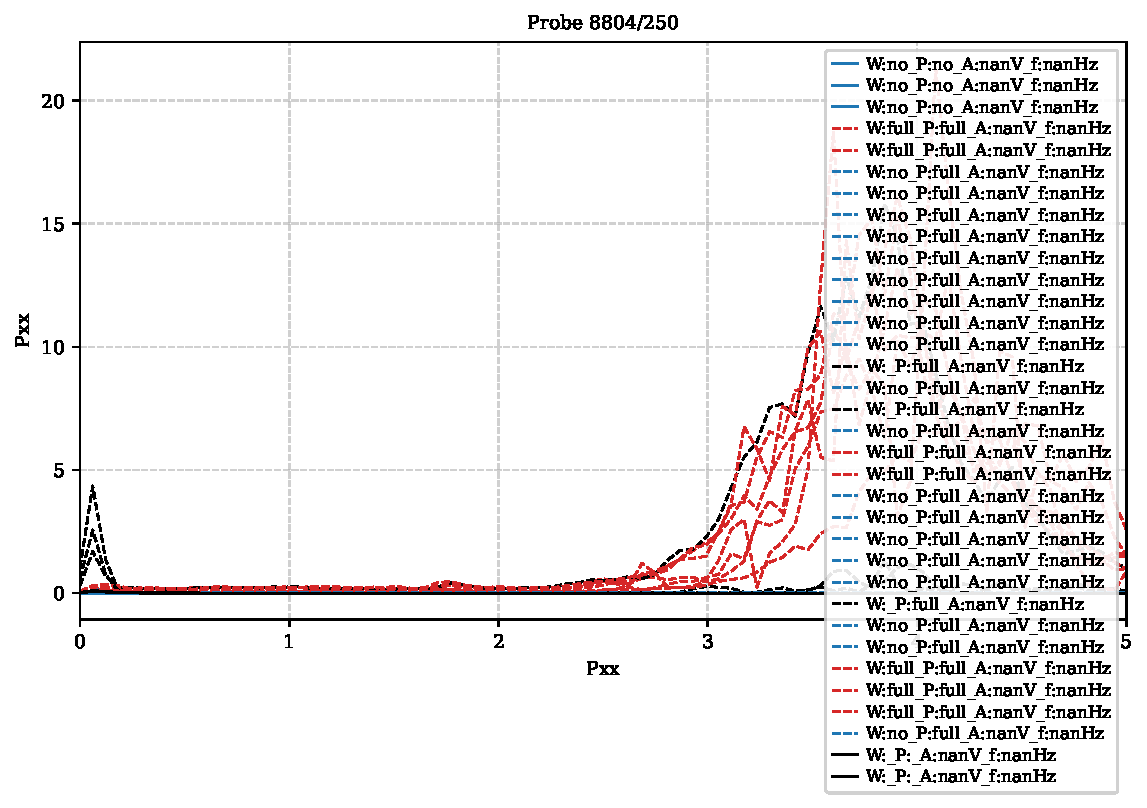
\includegraphics[width=\linewidth]{FIGURES/ch04_wind_psd.pdf}
    \caption{TODO}
    \label{fig:ch04_wind_psd}
  \end{subfigure}
  \hfill
  \begin{subfigure}[b]{0.48\linewidth}
    \centering
    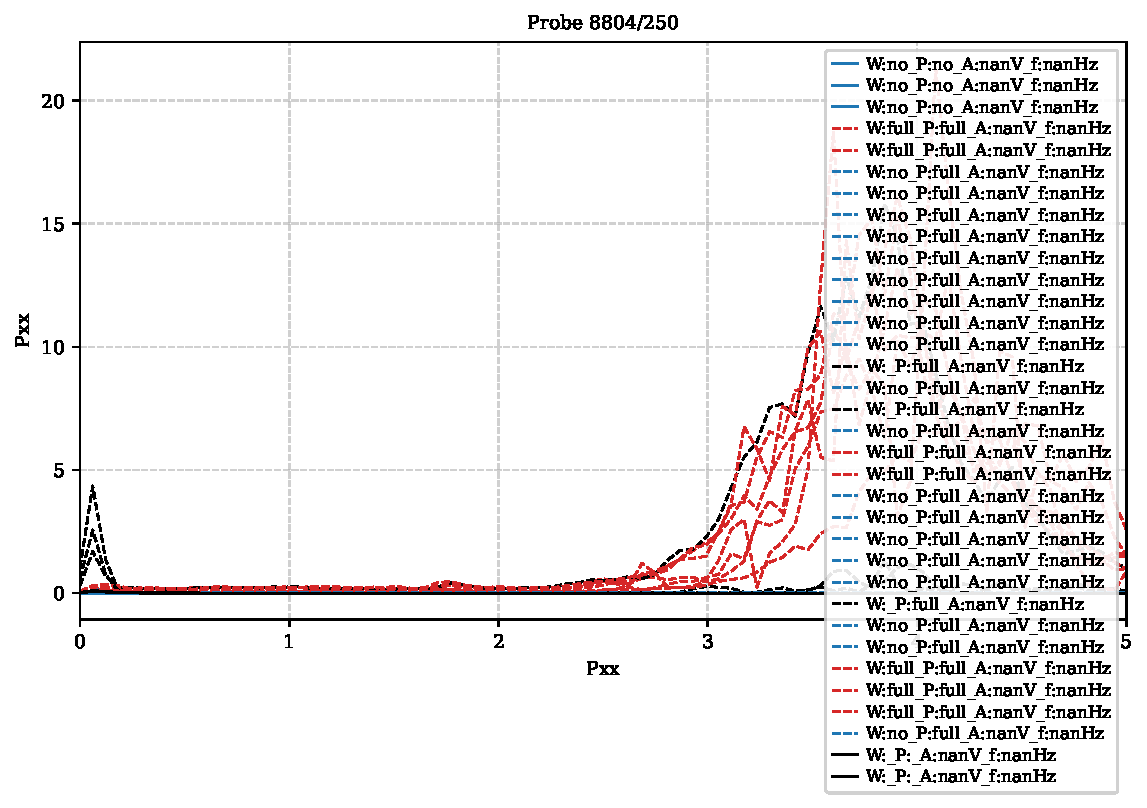
\includegraphics[width=\linewidth]{FIGURES/ch04_wind_psd.pdf}
    \caption{TODO}
    \label{fig:ch04_wind_psd}
  \end{subfigure}
  \caption{
    % TODO: write caption
  }
  \label{fig:ch04_wind_psd}
\end{figure}
